\documentclass[../notes.tex]{subfiles}

\graphicspath{{\subfix{../img/}}}

\begin{document}

\section{CSC473: Advanced Algorithms}

\subsection{Global Min-Cut (Karger's Contraction Algorithm)}


\textbf{Given} an undirected, unweighted, and connected graph $ G = (V, E) $, \textbf{return} the smallest set of edges that disconnects $ G $



\begin{figure}[H]
  \centering
  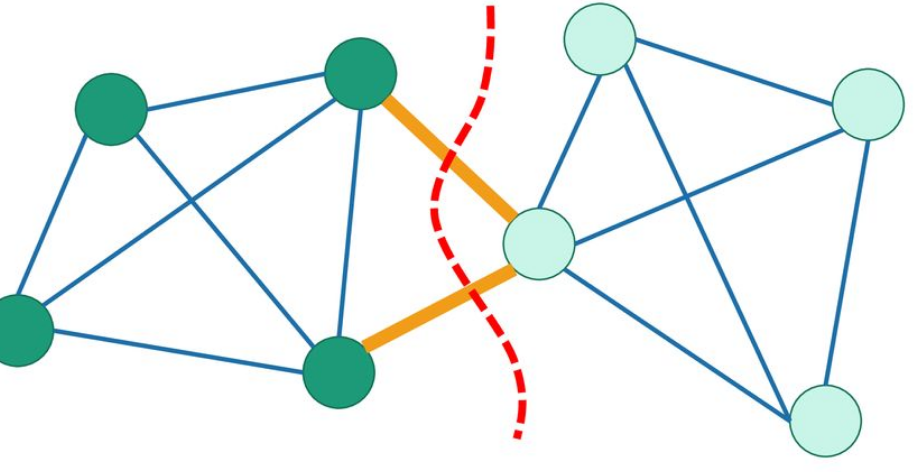
\includegraphics[width=0.8\linewidth]{img/image_2023-01-09-12-40-24.png}
  \caption{Example of global min-cut. Note that the global min-cut is not necessarily unique}
\end{figure}

\marginnote{An example of where this may be useful is in computer networks where we can measure the resiliency of a network by how many cuts must be made before a vertex (or many) get disconnected}


\begin{lemma}
  If the min cut is of size $ \ge k $, then $ G $ is $ k $-edge-connected
\end{lemma}

It may be more convenient to return a set of vertices instead

\begin{definition}
  
\begin{equation}
  S, T \subseteq V, S \cap T = \varnothing 
\end{equation}

\begin{equation}
  E(S,T) = \{(u,v) \in E : u \in S, v \in T\} 
\end{equation}

The global min-cut is to output $ S \subseteq V $ such that $ S \neq \varnothing, S \neq V $,  such that $ E(S, V\setminus S ) $ is minimized.


\end{definition}

\begin{blockquote}

Note that the min-cut-max-flow problem is somewhat of a dual to the global min-cut problem; the min-cut-max-flow problem imposes a few more constraints than the global min-cut algorithm i.e. having a directed and weighted graph as well as the notion of a source or sink.

\begin{itemize}
  \item \textbf{Input: }  Directed, weighted, and connected $ G = (V,E) $, $ s \in V, t \in V $
  \item \textbf{Output}  : $ S $ such that $ s \in S, t \notin S $ such that $  |E(S, V\setminus S ) |  $ is minimized
\end{itemize}
  
\end{blockquote}

We can kind of intuitively see that the global min-cut can be taken to the minimum of all max-flows across the graph.
So we can take the max-flow solution and then reduce it to find the global min cut.

Question: how many times will we have to run max-flow to solve the global min-cut problem? 
Naively, we may fix $ t $ to be an arbitrary node, then try every other $ s \neq t $ to find the $  s-t $ min-cut to get the best global min-cut.

We know from previous courses that the Edmonds-Karp max-flow algorithm will run in $ O(nm^2) = O(n^5) $, which makes our global min-cut algorithm $ O(n^6) $.
However, there is a paper recently published which gives an algorithm for min-cut in nearly linear time, i.e $ O(m^{1-O(1)}) = O(n^2) $  which gives a global min-cut runtime of $ O(n^3) $.

A randomized algorithm will be presented that solves this problem in $ O(n^2 \log^2 n) $


\begin{definition}
  The \textbf{Contraction} operation takes an edge $ e = (u,v) $ and \textit{contracts} it into a new node $ w $ such that all edges connected to $ u,v $ now connect to $ w $ and $ u,v $ are removed. Note that the contracted nodes can be supernodes themselves.

  \begin{figure}[H]
    \centering
    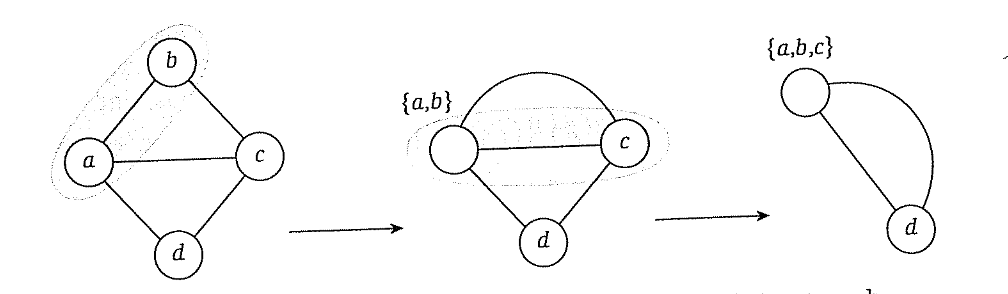
\includegraphics[width=0.8\linewidth]{img/image_2023-01-12-16-47-50.png}
    \caption{Example of a series of contractions}
  \end{figure}

\end{definition}


\begin{codebox}
\Procname{$\proc{contraction}(G=(V,E))$}
\li \While $ G $ has more than 2 supernodes
\li Pick an edge $ e = (u,v) $ uniformly at random
\li Contract $ e $, remove self-loops
\li Output the cut $ (S, V \setminus S )$ corresponding to the two super nodes \End
\end{codebox}

The contraction algorithm then recurses on $ G' $, choosing an edge uniformly at random and then contracting it. 
The algorithm terminates when it reaches \textit{a} $ G' $ with only two supernodes $ v_1, v_2 $. 
The sets of nodes contracted to form each supernode $ S(v_1), S(v_2) $ form a partition of $ V $ and are the cut found by the algorithm.



\subsubsection{Analysis}

The algorithm is still random, so there's a chance that it won't find the real global min-cut. 
With some analysis we will show that the success polynomial is not exponential as one may think, but really only polynomially small.
Therefore by running the algorithm a polynomial number of times and returning the best cut identified we can find a global min-cut with high probability.


\begin{lemma}
  The contraction algorithm returns a global min cut with probability at least $ \frac{1}{\binom{n}{2}} $
  \begin{proof}
    Take a global min-cut $ (A, B) $ of $ G $ and suppose it has size $ k $, i.e. there is a set $ F $ of $ k $ edges with one end in $ A $ and the other in $ B $.
    If an edge in $ F $ gets contracted then a node of $ A$ and a node in $ B $ would get contracted together and then the algorithm would no longer output $ (A, B) $, a global min-cut.
    An upper bound on the probability that an edge in $ F $ is contracted is the ratio of $ k $ to the size of $ E $. A lower bound on the size of $ E $ can be imposed by noting that if any node $ v $ has degree $ < k $ then $ ({v}, V\setminus {v}) $ would form a cut of size less than $ k $ -- which contradicts our first assumption that $ (A,B) $ is a global min-cut.
    So the probability than an edge in $ F $ is contracted at any step is

    \begin{equation}
      \frac{k}{(\frac{k}{2})} = \frac{2}{n}
    \end{equation}
    Note that here we use the number of vertices instead of the number of edges since each contraction removes (combines) one vertex, whereas since the amount of edges after a contraction can be very difficult to calculate.

    Next, let's inspect the algorithm after $ j $ iterations. 
    There will be $ n-j $ supernodes in $ G' $ and we can take that no edge in $ F $ has been contracted yet. 
    Every cut of $ G' $ is a cut of $ G $, so there are at least $ k $ edges incident to every supernode of $ G' $\mn{since the min-cut has $ k $ edges}. Therefore $ G' $ has at least $ \frac{1}{2}k(n-j) $ edges, and so the probability than an edge of $ F $ is contracted in $ j+1 $ is at most
    \marginnote{In terms of edges, it would be $ \frac{k}{m_{i-1}} $, but again, edges are difficult to work with so we'll do it w.r.t the vertices/supernodes}

    \begin{equation}
      \frac{k}{\frac{1}{2}k(n-j)} = \frac{2}{n-j}
    \end{equation}


  \begin{equation}
    P(A_i | A_1\ldots_{i-1}) \ge \frac{n-i-1}{n-i+1} = 1 - \frac{2}{n-i+1}
  \end{equation}


  The global min-cut will be actually returned by the algorithm if no edge of $ F $ is contracted in iterations $  1 - n $.

  What we want to know, then, is what is the probability of this algorithm never making a mistake?


  \marginnote{This prof uses commas to indicate intersection...}
  \begin{equation}
    P(A_1 \ldots A_{n-1}) = P(A_1)P(A_2 | A_1) P(A_3 | A_1, A_2) \ldots P(A_{n-2} | A_1, A_2, \ldots, A_{n-3})
  \end{equation}

  From what we found previously we know that this is 

  \begin{equation}
    \ge \frac{n-2}{n} \times \frac{n-3}{n-1} \times \frac{n-4}{n-2} \ldots \times \frac{2}{4} \times \frac{1}{3}  = \frac{2}{n(n-1)} =  \frac{1}{\binom{n}{2}}
  \end{equation}

  \end{proof}

  This gives us a bound of $ O(n^2) $ using the $ n^2 $ term from the number of contractions and then $ n^2 $ to get correct output with constant probability of success.

\end{lemma}


The key observation is that early contractions are much less likely to lead to a mistake, which leads us to the Karger-Stein min cut. 

\subsection{Karger-Stein Min Cut Algorithm}

This algorithm solves the global min-cut problem in $ O(n^2 \log^2 n) $ by taking advantage of the earlier cuts; it stops the contraction algorithm after an arbitrary fraction of contractions steps and then recursively contracts \textit{more carefully}.

Exercise: show the following:


The probability of no mistake in the first $ i $ contractions
\begin{equation}
  P(A_1, A_2, \ldots A_i) \ge \frac{(n-i)(n-i-1)}{n(n-1)}
\end{equation}


\begin{codebox}
\Procname{$\proc{min-cut}(G = (V,E))$}
\li \If $ G $ has two supernodes corresponding to $ S, \hat{S} $ \Then
\li   \Return $ S, \hat{S} $\End 
\li Run the contraction algorithm until $ \frac{n}{\sqrt{2} } + 1 $ supernodes remain
\li Let $ G' $ be the resulting contracted multigraph
\li $ (S_1, \hat{S_1}) = \proc{min-cut}(G') $
\li $ (S_2, \hat{S_2}) = \proc{min-cut}(G') $
\li \Return the cut ($ S_i, \hat{S_i}$) with the smaller number of edges
\end{codebox}

\begin{theorem}
  $ \proc{Min-cut}(G) $ runs in $ O(n^2) \log n $ and outputs a min cut of $ G $ with probability of at least $ \frac{1}{O(\log n)} $\mn{So repeat the algorithm $ O(\log(n)) $ times, leading to $ O(n^2 \log^2 n) $ runtime} 


  \begin{proof}
      The intuition for this can be developed by drawing out a recursion tree for this problem.
      At each level the number of recursive call doubles, but the time it takes for each sub-call halves as well.
      This means that the total runtime for each level is $ n^2 $. 
      As for the total time will just be $ O(n^2 \log (n))$, since we know the height of the recursion tree to be $ \log n $.


      More formally, the recursion may be described with 

      \begin{equation}
          T(n) \le  2T(\frac{n}{\sqrt{2} } + O(n^2))
      \end{equation}

      Which can \mn{I think? } be solved with the master theorem.
      
  \end{proof}
  


\end{theorem}

We may also want to understand the probability of success.

\begin{itemize}
    \item We may deem a node in the recursion tree to be \textit{successful} if it survives the contractions.
        \begin{itemize}
            \item There must be a leaf node in a recursion tree that successfully produces a min-cut that corresponds to a min-cut, therefore there must also be a sequence of \textit{successful} nodes from the root to said min cut.
        \end{itemize}
    \item $ P(d) $ as the probability that a node at depth d is successful, conditioned on it's ancestors being successful
\end{itemize}

Now, how can we find $ P(h) $? I.e. the probability of the algorithm being successful on termination.
\begin{itemize}
    \item Base case: $ P(0) \ge \frac{1}{2} $ (will assume $ = \frac{1}{2} $, worst case)
    \item Inductive step: $ P(D) = \frac{1}{2} ( 1- (1-(P(d-1)))^2 ) = \frac{1}{2} (2P(d-1) - P(d-1)^2) $ 
      \begin{itemize}
        \item At each level the probability of success is at least $ \frac{1}{2}$, conditioned on the ancestors being successful.
      \end{itemize}
\end{itemize}

What remains now is solving this recursion.


\begin{equation}
  P(d) = P(d-1) - \frac{1}{2} P(d-1)^2
\end{equation}

The way of solving a non-linear recursion is to make a guess.
We expect this to be on the order of

\begin{equation}
  P(d) \ge  \frac{1}{d}
\end{equation}

And then as it turns out it's 

\begin{equation}
  P(d) = \frac{1}{d+2}
\end{equation}

And then this can be checked by doing an induction proof














\begin{blockquote}
  Note that there are two types of randomized algorithms:
  \begin{itemize}
    \item Monte carlo algorithms: bound on worst-case time \& produces a correct answer with a probability $ \ge  $ some constant
    \item Las vegas algorithms: bound on the expected value of running time, but the output is always correct
  \end{itemize}

  Our contraction algorithm is a monte-carlo algorithm
\end{blockquote}














\end{document}
